\documentclass[eng]{class}

% Publication Title
\title{EDI: Third Lab Report}
% Short title for the header (copy the main title if it is not too long)
\shorttitle{Third Lab Report}
       
% Authors
\author[1]{D. Ligari 518592}
% Author Affiliations
\affil[1]{University of Pavia, Department of Computer Engineering (Data Science), Pavia, Italy}
% Surname of the first author of the manuscript
\firstauthor{Ligari}
%Contact Author Information
\contactauthor{D. Ligari} % Name and surname of the contact author
\email{davide.ligari01@universitadipavia.it} % Contact Author Email
% Publication data (will be defined in the edition)
\publicationdate{\today}
% Place your particular definitions here
\newcommand{\vect}[1]{\mathbf{#1}}  % vectors
\github{https://github.com/DavideLigari01/Enterprise-Digital-Infrastructure}

\abstract{
  This report examines the impact of web technologies on Page Load Times (PLTs) for commercial and institutional websites. 
  It analyzes parallel connections, caching policies, and performance evaluation tools. The findings highlight the significance of parallel connections, 
  the effects of caching policies on PLTs, and provide insights for optimizing website performance. 
  The report also evaluates website performance under different conditions and explores the role of warm-up time.}
\keywords{HTTP cache policies • HTTP • PLT • Apache HTTP server benchmarking tool • h2load}
\date{\today}
% Start document
\begin{document}
\pagenumbering{arabic}
% Include title, authors, abstract, etc.
\maketitle
\tableofcontents
\thispagestyle{FirstPage}

\section{Introduction}
\firstword{I}{n}
today's digital landscape, web technologies play a pivotal role in determining the performance and overall user experience of modern websites.
As the internet continues to evolve and user expectations rise, it becomes increasingly crucial to understand the profound impact
that these technologies have on Page Load Times (PLTs) for commercial and institutional websites.\\
This report aims to delve into various aspects of web technologies,
exploring their effects on PLTs and providing valuable insights to optimize website performance.

\section{Impact of parallel connections on PLTs}
\subsubsection*{Analyze and discuss the impacts of the number of parallel connections set inside the browser
	on the Page Load Times of commercial/institutional websites. Did you notice any expected or
	unexpected behavior?}
The impact of increasing the number of connections on page loading time is evident and consistent, as depicted in Figure \ref{fig-1}.
Experimental results clearly demonstrate that as the number of connections increases, the loading time consistently decreases,
showcasing the advantage of parallel downloading.
This effect can be attributed to the browser's ability to simultaneously download multiple files, resulting in an overall improvement in download speed.\\
However, it's important to note that the relationship between the number of connections and loading time is influenced by the size of the webpage.
For smaller page sizes, exemplified by the website \textit{www.pedranzini.it/}, the loading time remains relatively consistent regardless
of the number of connections. This suggests that the page can be efficiently loaded with a limited number of connections due to its compact size.
The downloading process for such pages is optimized, and further increasing the number of connections does not significantly impact the loading time.\\
Conversely, for larger page sizes, such as the case of \textit{www.vallespluga.it/}, the loading time exhibits a significant decrease as
the number of connections increases. This indicates that the page benefits from parallel connections to efficiently download its extensive content.
As the page size increases, the impact of parallel connections on reducing loading time becomes more pronounced.\\
To provide additional context, the table below presents the websites used for the analysis, along with their respective characteristics.
\rowcolors{2}{purple!8}{purple!18}
\begin{table}[H]
	\tiny
	\centering
	\begin{tabular}{|c|c|c|c|c|c|}
		\hline
		\linewidth=0cm
		Website             & Page size(KB) & Cache policy            & HTTP version & HTTPS         \\
		\hline
		www.pedranzini.it/  & 180.40        & Validation              & 1.1          & Not supported \\
		www.unica.it/       & 2570          & Validation              & 1.1          & Supported     \\
		www.uniss.it/       & 2540          & Validation • Expiration & 1.1          & Supported     \\
		www.vallespluga.it/ & 20120         & Validation              & 1.1          & Supported     \\
		\hline
	\end{tabular}
	\caption{Website used for the analysis}
	\label{tab-1}
\end{table}
\begin{figure}[H]
	\centering
	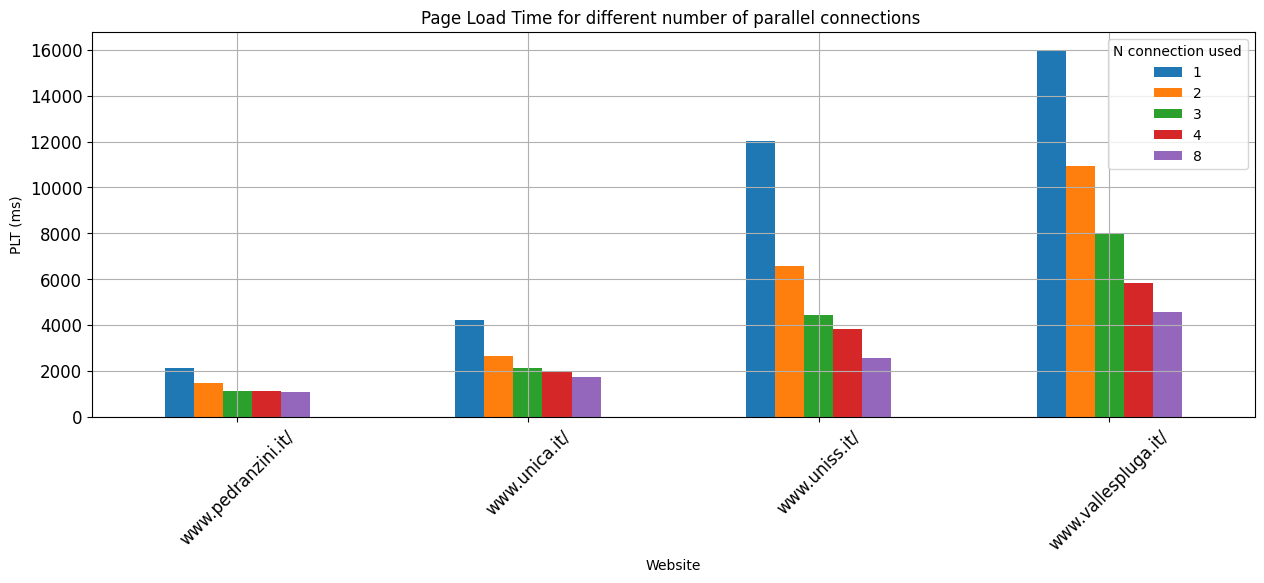
\includegraphics[width=0.8\columnwidth]{images/plt_vs_conc_1.1.png}
	\caption{Page load time vs number of concurrent connections for different sites}
	\label{fig-1}
\end{figure}

\pagestyle{OtherPage}
\section{Impact of caching policies on PLTs}
\subsubsection*{Analyze and discuss the impacts of caching policies implemented by different
	commercial/institutional websites on the Page Load Times. Consider websites that support
	HTTP/1.1, HTTP/2 and HTTP/3 (possibly with unsecure and secure connections). Did you notice
	any expected or unexpected behavior?}

To provide a comprehensive understanding, an extensive analysis was conducted on multiple websites with varying characteristics, as presented in Table \ref{tab-2}.
Thorough testing was ensured by evaluating sites that supported multiple versions of the HTTP protocol with each version.\\
Upon examining the results depicted in Figure \ref{fig-2}, a noteworthy observation emerges: websites supporting HTTP/2 or HTTP/3
consistently exhibit faster loading times compared to those supporting only HTTP/1.1, regardless of the implemented cache policy.
This finding underscores the undeniable performance benefits associated with the adoption of newer HTTP protocol versions.\\
Furthermore, the analysis sheds light on the impact of different cache policies.
Websites supporting both validation and expiration cache policies were found to have shorter loading times compared to those supporting only the validation policy.
This outcome can be attributed to the combined advantages of validating cached content and leveraging expiration times to minimize server requests.
In contrast, websites lacking any caching mechanism displayed higher Page Load Times (PLTs),
underscoring the crucial role of effective caching in optimizing web performance.\\
Considering that page load time is significantly influenced by page size, and the analyzed pages vary in size,
the values displayed in Figure \ref{fig-2} have been normalized accordingly.
Additionally, it is important to note that the analyzed sites contain objects served by different servers,
resulting in requests using different versions of HTTP and cache policies. To address this issue,
each site was assigned the most commonly used HTTP cache policy and protocol.

\rowcolors{2}{purple!8}{purple!18}
\begin{table}[H]
	\tiny
	\centering
	\begin{tabular}{|c|c|c|c|c|}
		\hline
		\linewidth=0cm
		Website              & Page size(KB) & Cache policy            & HTTP version & HTTPS         \\
		\hline
		www.pedranzini.it/   & 180.40        & Validation              & 1.1          & Not supported \\
		www.unica.it/        & 2570          & Validation              & 1.1          & Supported     \\
		www.uniss.it/        & 2540          & Validation • Expiration & 1.1          & Supported     \\
		www.vallespluga.it/  & 20120         & Validation              & 1.1          & Supported     \\
		www.istat.it/        & 11200         & Validation              & 1.1          & Supported     \\
		www.unina.it/        & 2210          & Validation              & 1.1          & Supported     \\
		www.apache.org/      & 2010          & Validation • Expiration & 3            & Supported     \\
		www.studiocamer.com/ & 3340          & Validation • Expiration & 2 • 3        & Supported     \\
		www.off---white.com/ & 6790          & Validation              & 1.1 • 2 • 3  & Supported     \\
		www.google.com       & 2350          & Validation • Expiration & 1.1 • 2 • 3  & Supported     \\
		\hline
	\end{tabular}
	\caption{Website used for the analysis}
	\label{tab-2}
\end{table}

\begin{figure}[H]
	\centering
	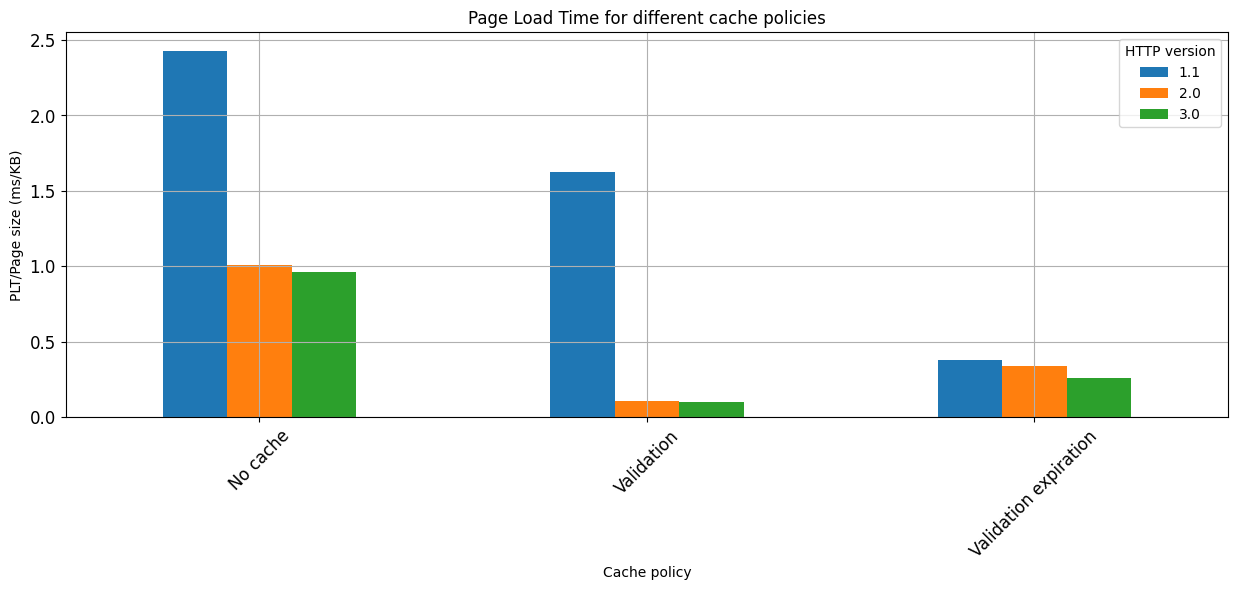
\includegraphics[width=\columnwidth]{images/plt_cache_policy.png}
	\caption{Page load time over page size for different cache policies for different HTTP versions}
	\label{fig-2}
\end{figure}

\section{Performance analisys using  Apache HTTP server benchmarking tool}
Ab (ApacheBench), it is a command-line tool that comes bundled with the Apache HTTP Server.
It is designed to perform load testing and measure the performance of web servers.
The "ab" tool allows users to simulate multiple concurrent requests to a web server and record various performance metrics,
such as requests per second, latency, and throughput.
Below an example of the command used to perform the analysis, where the number of concurrent connections is set to 2 and the number of requests to 30.
\begin{lstlisting}
  ab -c 2 -n 30 www.galbusera.it/chi-siamo/
\end{lstlisting}

\subsubsection*{Analyze and discuss the performance of different commercial/institutional websites obtained
	under different conditions using the ab – Apache HTTP server benchmarking tool. Did you
	notice any expected or unexpected behavior?}
The websites listed in Table \ref{tab-3} were subjected to analysis using the 'ab' command to evaluate their performance under different conditions.
Specifically, the impact of concurrency level on requests per second and transfer rate was assessed, as depicted in Figure \ref*{fig-3} and \ref*{fig-4} respectively.
The results indicate that increasing the concurrency level leads to higher requests per second and transfer rate,
aligning with the findings discussed in Section 1.a, where an increase in the number of connections resulted in decreased page load time.\\
However, there were some unexpected results observed for certain websites. For instance, \textit{www.galbusera.it/chi-siamo/}
exhibited a slight decrease in transfer rate and requests per second when transitioning from 4 to 8 connections.
This anomaly could be attributed to factors like server congestion or limited network bandwidth at 8 connections.
However, with 16 connections, network congestion might be alleviated, potentially improving performance.
Alternatively, the website's server infrastructure might incorporate load balancing mechanisms that distribute requests evenly across
a limited number of resources, causing a slight decrease in performance with 4 to 8 connections but optimizing resource allocation with 16 connections.\\
Another anomalous finding was observed for \textit{www.pedranzini.it/}, which displayed a significantly higher number of
requests per second compared to other websites but a lower transfer rate. This outcome can be attributed to the smaller size of the website,
resulting in a higher number of requests per second despite the server's relatively lower performance in terms of transfer rate.\\
\noindent
To gain further insights, an additional analysis was conducted to evaluate the time distribution across the connecting, processing, and waiting phases,
as depicted in Figure \ref*{fig-5}.
The results illustrate that the time spent on the connection phase is relatively minimal when compared to the time allocated to processing and waiting.\\
The graphs clearly demonstrate that the majority of time is dedicated to processing the request on the server and waiting for the necessary operations to be completed.
This observation highlights the significance of server-side computations and any external dependencies involved in generating the response.
The processing phase, which encompasses executing server-side scripts, performing database queries,
or conducting complex computations, typically consumes a substantial portion of the overall time.\\
Intriguingly, the waiting time, during which the server may be accessing external resources or performing additional computations
before generating the complete response, is found to be lower than the processing time. This suggests that the waiting phase is generally efficient,
possibly due to optimized resource access or caching mechanisms employed by the server.
\rowcolors{2}{purple!8}{purple!18}
\begin{table}[H]
	\tiny
	\centering
	\begin{tabular}{|c|c|c|c|c|}
		\hline
		\linewidth=0cm
		Website                     & Page size(KB) & Cache policy            & HTTP version & HTTPS         \\
		\hline
		www.pedranzini.it/          & 180.40        & Validation              & 1.1          & Not supported \\
		www.vallespluga.it/         & 20120         & Validation              & 1.1          & Supported     \\
		www.galbusera.it/chi-siamo/ & 15610         & Validation • Expiration & 3            & Supported     \\
		\hline
	\end{tabular}
	\caption{Website used for the analysis}
	\label{tab-3}
\end{table}


\begin{figure}[H]
	\centering
	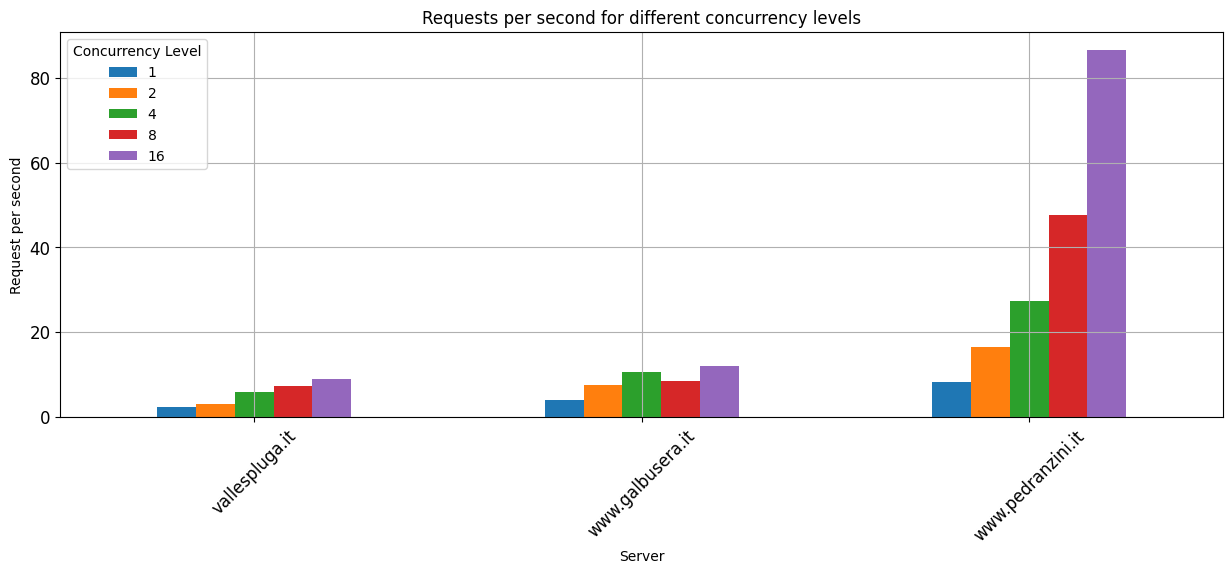
\includegraphics[width=\columnwidth]{images/Request_per_second_diff_conc.png}
	\caption{Number of request per second for different number of concurrent connections for different sites}
	\label{fig-3}
\end{figure}
\begin{figure}[H]
	\centering
	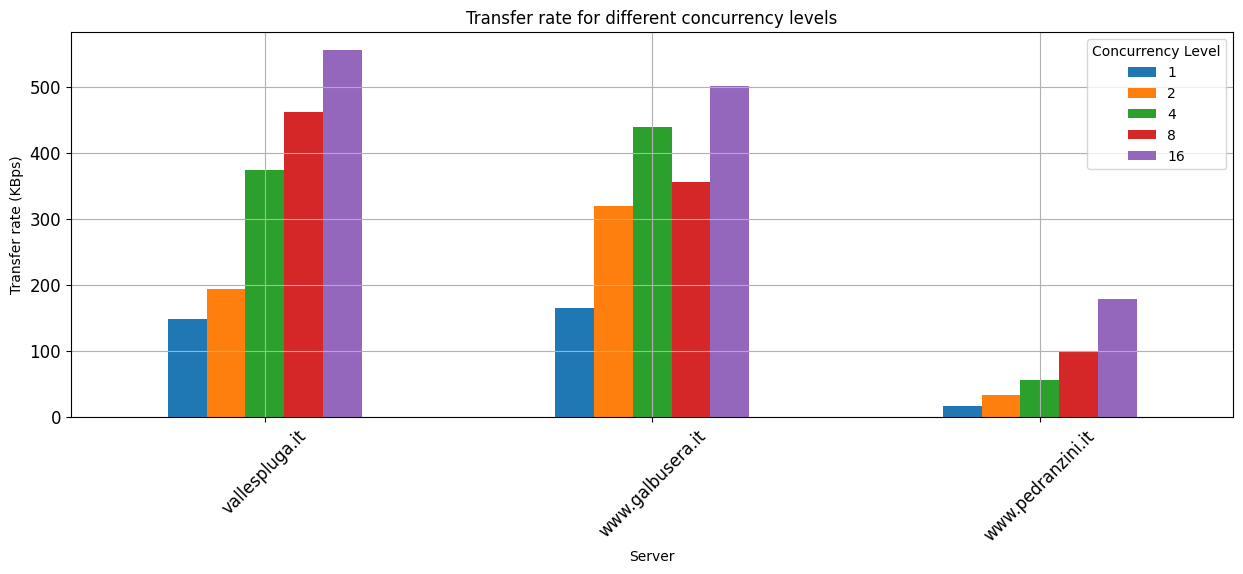
\includegraphics[width=\columnwidth]{images/transf_diff_conc.png}
	\caption{Transfer rate for different number of concurrent connections for different sites}
	\label{fig-4}
\end{figure}

\begin{figure}[H]
	\centering
	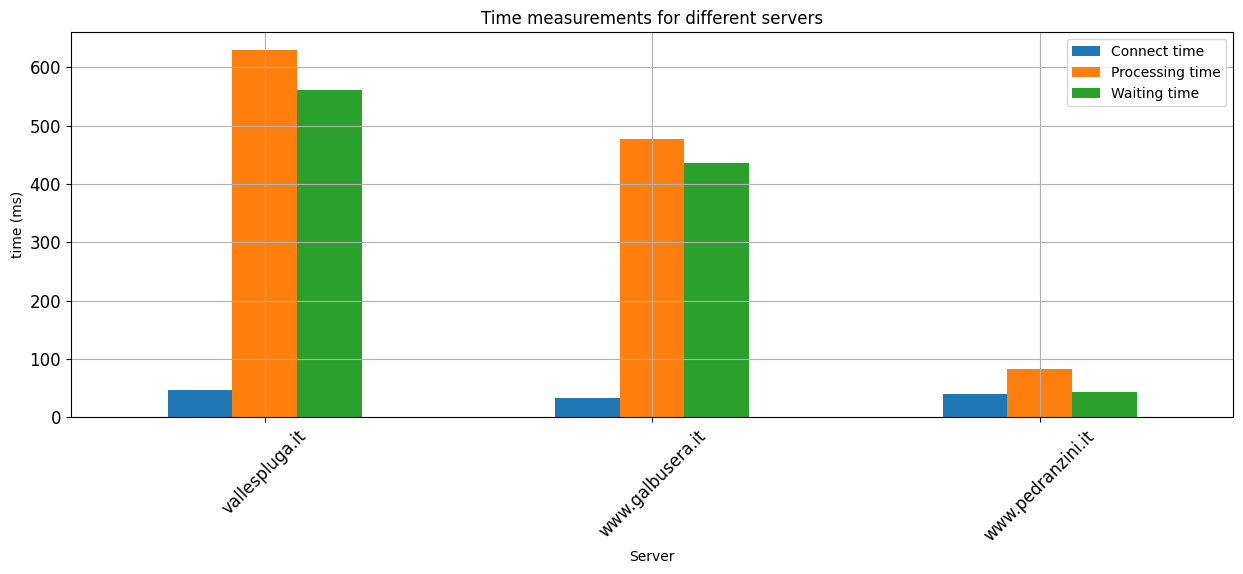
\includegraphics[width=\columnwidth]{images/time_diff_server.png}
	\caption{Time spent for the connection, for processing and for waiting for different sites}
	\label{fig-5}
\end{figure}

\section{Performance analisys using h2load}

h2load is a command-line benchmarking tool specifically designed for testing the performance of HTTP/2 and HTTP/3 servers.
It is part of the nghttp2 project, which focuses on developing and maintaining tools and libraries for working with HTTP/2 and HTTP/3 protocols.
h2load allows you to simulate a large number of concurrent requests to a server and measure its performance under various conditions.
It can be used to assess the server's capability to handle a high volume of traffic, evaluate response times, measure throughput,
and identify potential bottlenecks or performance issues.
Below an example of usage.
\begin{lstlisting}
  h2load --duration=30 -c 16 --warm-up-time=4  https://www.galbusera.it/chi-siamo/
\end{lstlisting}

\section{The role of Warm up time}
The warm-up time in h2load plays an important role in ensuring accurate performance measurements that reflect the server's stable behavior under load.\\
The introduction of the warm-up phase is motivated by the fact that at the beginning of a load test, the server and the network environment may be in a transient state. 
This means that network connections may take time to establish, cache systems may require population, or server resources may be dynamically allocated.\\
These factors can influence the initial requests sent to the server and produce results that are not representative of 
its actual performance once it reaches a stable state. 
The warm-up phase helps address this issue by allowing the system to stabilize before measuring the actual performance.\\
In essence, the warm-up phase enables more reliable and realistic measurements of the server's performance. 
By eliminating the effects of transient factors, it ensures that the measurements reflect the server's true potential when subjected to a steady workload.


\subsubsection*{Analyze and discuss the performance of different commercial/institutional websites obtained
	under different conditions using the nghttp and h2load tools. In the experiments with
	h2load analyze the role of the warm-up time. Did you notice any expected or unexpected
	behavior?}
To analyze the role of warm-up time, performance tests were conducted using h2load.
The tests were designed to measure the impact of warm-up time and the number of connections on website performance.
Each test ran for 30 seconds, varying the number of connections and warm-up times at 1, 2, 4, 8, and 16.\\
Multiple websites were included in the analysis, ensuring a diverse range of warm-up times and connection settings.
The obtained results were evaluated in terms of transfer rate, mean time, and standard deviation.\\
Examining the transfer rate and mean time results, as displayed in Figure \ref{fig-6} and \ref{fig-7} respectively,
it appears that warm-up time does not have a significant impact on these metrics.
However, when analyzing the standard deviation, as shown in Figure \ref{fig-8}, it becomes evident that warm-up time plays a significant role.\\
For most connection levels, a longer warm-up time corresponds to a lower standard deviation, with a warm-up time of 8 seconds exhibiting the lowest deviation.
On the other hand, longer warm-up times lead to higher standard deviations. \\
However, a different pattern emerges when considering a connection level of 16, where the standard deviation decreases with increasing warm-up time.\\
These findings suggest that warm-up time can have varying effects on performance depending on the number of connections.
While it does not significantly impact the transfer rate and mean time, it can contribute to reducing the variability of response times,
indicated by the standard deviation. The relationship between warm-up time and performance metrics can be complex,
influenced by factors such as server caching, resource availability, and network conditions.
Further analysis and experimentation are necessary to understand the underlying reasons behind these observed results and their broader implications.
\rowcolors{2}{purple!8}{purple!18}
\begin{table}[H]
	\tiny
	\centering
	\begin{tabular}{|c|c|c|c|c|}
		\hline
		\linewidth=0cm
		Website                     & Page size(KB) & Cache policy            & HTTP version & HTTPS     \\
		\hline
		www.youtube.com/            & 14050         & Validation • Expiration & 1.1          & supported \\
		www.reddit.it/              & 17360         & Validation              & 2            & Supported \\
		www.regionelombardia.it/    & 13580         & Validation • Expiration & 1.1          & Supported \\
		www.galbusera.it/chi-siamo/ & 15610         & Validation • Expiration & 3            & Supported \\
		\hline
	\end{tabular}
	\caption{Website used for the analysis}
	\label{tab-4}
\end{table}

\begin{figure}[H]
	\centering
	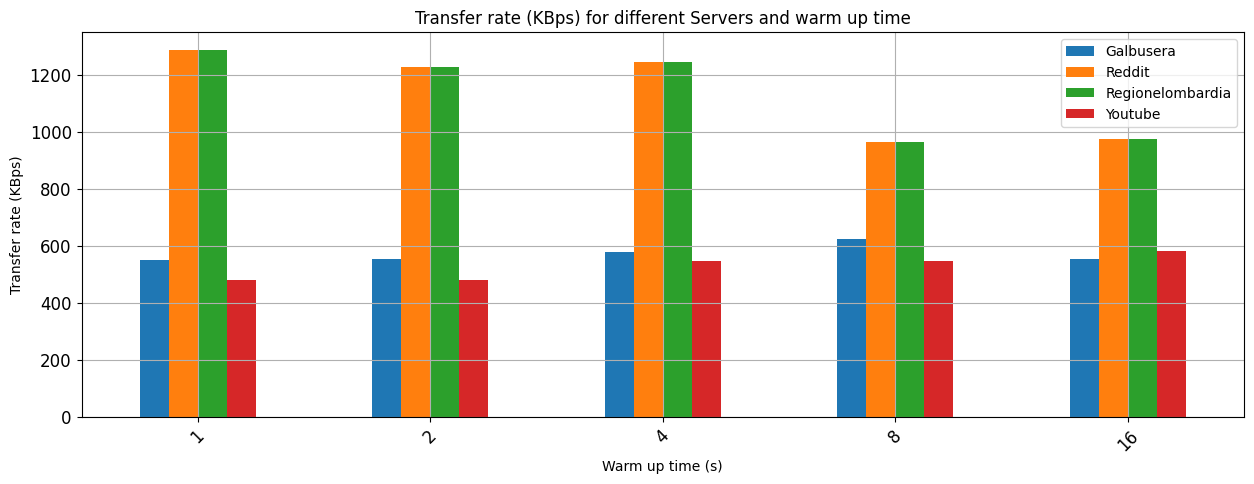
\includegraphics[width=\columnwidth]{images/transf_rate_diff_warm_up.png}
	\caption{Transfer rate for different warm up time for different sites}
	\label{fig-6}
\end{figure}

\begin{figure}[H]
	\centering
	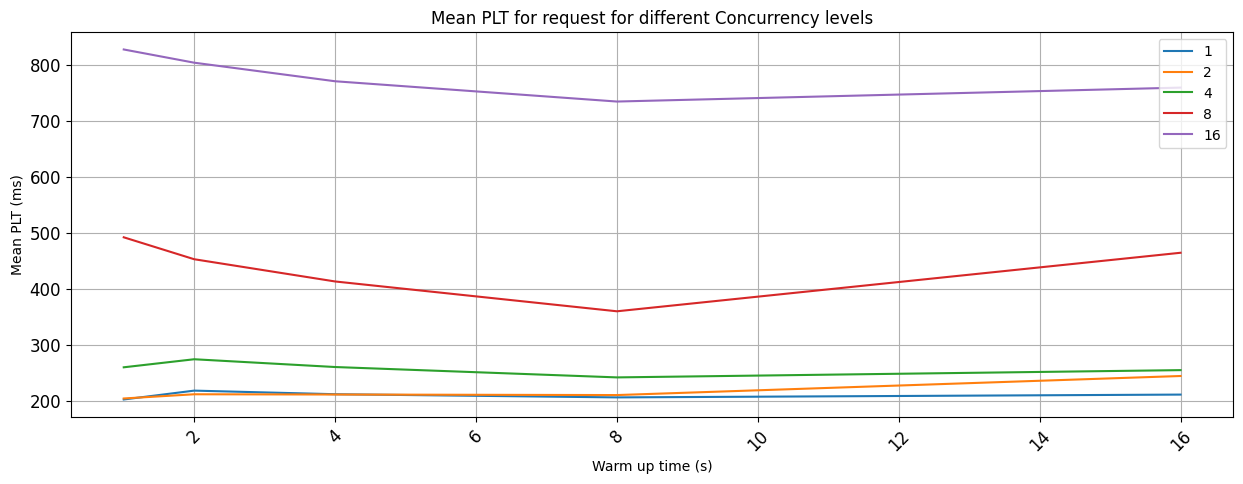
\includegraphics[width=\columnwidth]{images/mean_time_warm_up.png}
	\caption{mean time for different warm up time for different concurrent connections}
	\label{fig-7}
\end{figure}

\begin{figure}[H]
	\centering
	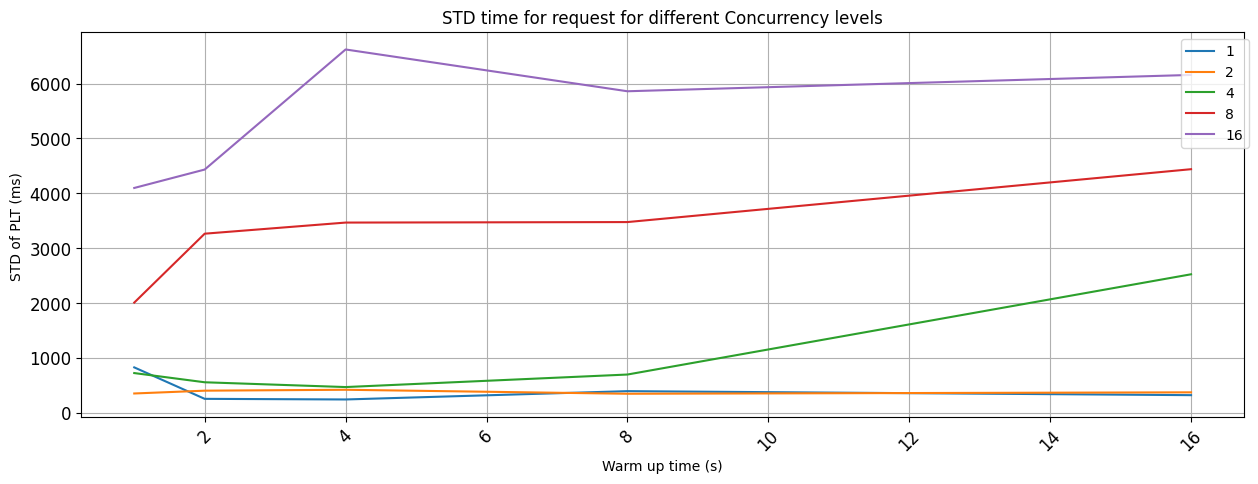
\includegraphics[width=\columnwidth]{images/var_warm_up.png}
	\caption{Standard deviation for different warm up time for different concurrent connections}
	\label{fig-8}
\end{figure}

\section{Conclusions}

In conclusion, this report has delved into the impact of web technologies on Page Load Times (PLTs) for commercial and institutional websites.
Through the analysis of parallel connections, caching policies, and performance evaluation tools, valuable informations have been gained regarding website optimization.\\
The findings indicate that increasing the number of parallel connections can significantly reduce loading times,
particularly for larger websites with extensive content. Additionally, websites supporting newer versions of the HTTP protocol,
such as HTTP/2 and HTTP/3, consistently exhibit faster loading times compared to those supporting only HTTP/1.1.
The implementation of effective caching policies, including both validation and expiration mechanisms,
has also been shown to contribute to shorter PLTs.\\
However, it is important to note that these analyses alone are not sufficient to draw definitive conclusions.
The performance of a website is influenced by various factors, including server configuration, network conditions, and user behavior.
Further research and experimentation are necessary to gain a more comprehensive understanding of web technologies'
impact on PLTs and to develop effective optimization strategies.

\end{document}